\documentclass{article}\usepackage[]{graphicx}\usepackage[]{xcolor}
% maxwidth is the original width if it is less than linewidth
% otherwise use linewidth (to make sure the graphics do not exceed the margin)
\makeatletter
\def\maxwidth{ %
  \ifdim\Gin@nat@width>\linewidth
    \linewidth
  \else
    \Gin@nat@width
  \fi
}
\makeatother

\definecolor{fgcolor}{rgb}{0.345, 0.345, 0.345}
\newcommand{\hlnum}[1]{\textcolor[rgb]{0.686,0.059,0.569}{#1}}%
\newcommand{\hlsng}[1]{\textcolor[rgb]{0.192,0.494,0.8}{#1}}%
\newcommand{\hlcom}[1]{\textcolor[rgb]{0.678,0.584,0.686}{\textit{#1}}}%
\newcommand{\hlopt}[1]{\textcolor[rgb]{0,0,0}{#1}}%
\newcommand{\hldef}[1]{\textcolor[rgb]{0.345,0.345,0.345}{#1}}%
\newcommand{\hlkwa}[1]{\textcolor[rgb]{0.161,0.373,0.58}{\textbf{#1}}}%
\newcommand{\hlkwb}[1]{\textcolor[rgb]{0.69,0.353,0.396}{#1}}%
\newcommand{\hlkwc}[1]{\textcolor[rgb]{0.333,0.667,0.333}{#1}}%
\newcommand{\hlkwd}[1]{\textcolor[rgb]{0.737,0.353,0.396}{\textbf{#1}}}%
\let\hlipl\hlkwb

\usepackage{framed}
\makeatletter
\newenvironment{kframe}{%
 \def\at@end@of@kframe{}%
 \ifinner\ifhmode%
  \def\at@end@of@kframe{\end{minipage}}%
  \begin{minipage}{\columnwidth}%
 \fi\fi%
 \def\FrameCommand##1{\hskip\@totalleftmargin \hskip-\fboxsep
 \colorbox{shadecolor}{##1}\hskip-\fboxsep
     % There is no \\@totalrightmargin, so:
     \hskip-\linewidth \hskip-\@totalleftmargin \hskip\columnwidth}%
 \MakeFramed {\advance\hsize-\width
   \@totalleftmargin\z@ \linewidth\hsize
   \@setminipage}}%
 {\par\unskip\endMakeFramed%
 \at@end@of@kframe}
\makeatother

\definecolor{shadecolor}{rgb}{.97, .97, .97}
\definecolor{messagecolor}{rgb}{0, 0, 0}
\definecolor{warningcolor}{rgb}{1, 0, 1}
\definecolor{errorcolor}{rgb}{1, 0, 0}
\newenvironment{knitrout}{}{} % an empty environment to be redefined in TeX

\usepackage{alltt}
\usepackage{amsmath} %This allows me to use the align functionality.
                     %If you find yourself trying to replicate
                     %something you found online, ensure you're
                     %loading the necessary packages!
\usepackage{amsfonts}%Math font
\usepackage{graphicx}%For including graphics
\usepackage{hyperref}%For Hyperlinks
\usepackage[shortlabels]{enumitem}% For enumerated lists with labels specified
                                  % We had to run tlmgr_install("enumitem") in R
\hypersetup{colorlinks = true,citecolor=black} %set citations to have black (not green) color
\usepackage{natbib}        %For the bibliography
\setlength{\bibsep}{0pt plus 0.3ex}
\bibliographystyle{apalike}%For the bibliography
\usepackage[margin=0.50in]{geometry}
\usepackage{float}
\usepackage{multicol}

%fix for figures
\usepackage{caption}
\newenvironment{Figure}
  {\par\medskip\noindent\minipage{\linewidth}}
  {\endminipage\par\medskip}
\IfFileExists{upquote.sty}{\usepackage{upquote}}{}
\begin{document}

\vspace{-1in}
\title{Lab 1 -- MATH 240 -- Computational Statistics}

\author{
  First Author \\
  Affiliation  \\
  Department  \\
  {\tt email@domain}
}

\date{}

\maketitle

\begin{multicols}{2}
\begin{abstract}
This document provides a basic template for the 2-page labs we will complete each week. Here, you should provide a succinct summary about what you did and why it might be helpful. 
\end{abstract}

\noindent \textbf{Keywords:} What topics does the lab cover with respect to the class?

\section{Instructions}
For this lab, you will \\ 


\begin{enumerate}
  \item Install \href{https://cran.rstudio.com}{R} and \href{https://posit.co/download/rstudio-desktop}{RStudio} 
  \item Install tinytex (if necessary): \\ install.packages("tinytex")
  \item Create a GitHub account \href{https://github.com}{here}, and email me your username.
  \item Install \href{https://github.com}{GitHub Desktop}.
  \item Accept the LAB 1 assignment \href{https://classroom.github.com/a/gfC_xMMl}{here}.
  \item Recreate this document (except put your name/info at the top) to get used to writing in \LaTeX~  and to see the types of things we can do when creating a document to convey statistical information. Make sure to commit and push your work using GitHub desktop as you finish each section.
\end{enumerate}

\noindent \textbf{Remarks:} You will find the class Sweave cheatsheet to be \emph{incredibly} \verb|\emph{incredibly}| helpful.

\section{Word Processing Tasks}
\subsection{Centering Text}
\begin{center}
We can center text in Sweave.
\end{center}
\subsection{Bold, Italics, and Underlining}
\noindent We can \textbf{bold}, \textit{italicize}, \underline{underline}, and \emph{emphasize} text in Sweave. \\
\indent Note, I did a column break here so that the list wasn’t broken across columns.

\columnbreak

\subsection{Lists, and Numbered Lists}
We can write an unordered list in Sweave.
\begin{itemize}
  \item first item
  \item second item
  \item third item
\end{itemize}

\noindent We can write an numbered list in Sweave.
\begin{enumerate}
  \item first item
  \item second item
  \item third item
\end{enumerate}

\noindent We can write an lettered list in Sweave.
\begin{enumerate}[a.]
  \item first item
  \item second item
  \item third item
\end{enumerate}



\subsection{Submissions}
This part of the midterm is due Sunday November 14 by 5p. I will not accept late submissions. Note that you may use this template to help build your introduction and methods sections, and you can use the work you did as a group during the datathon. Still, I expect this submission to be your own summary and extension of that work without collaboration.

\subsection{Typing Mathematical Equations}
We can write a one line equation that is centered like this
\begin{center}
  \[\widehat{y_i} = \beta_0 + \beta_1 x_{1i}+ \beta_2 x_{2i} + \epsilon_i.\]
\end{center}
This can be written in the text, as $\widehat{y_i} = \beta_0 + \beta_1 x_{1i}+ \beta_2 x_{2i} + \epsilon_i$ using as well.
  
When we need to show multiple steps, we can create a multi-line equation that is centered like this: 
\begin{align*}
8(x-5)+x&=9(x-5)+5 \\
8x-40+x&=9x-45+5 \tag{Distributing}\\
9x-40&=9x-40 \tag{Combining like terms}\\
9x&=9x \tag{Adding 40 to both sides}\\
9x&=9x \tag{Dividing both sides by 9}
\end{align*}
The equality holds for any x.

Note, I did a page break here so that the next section
started on a clean page.
\pagebreak

\subsection{Running R Code}
Code chunks can be entered into Sweave; e.g., here are some comments.

\begin{knitrout}\scriptsize
\definecolor{shadecolor}{rgb}{0.969, 0.969, 0.969}\color{fgcolor}\begin{kframe}
\begin{alltt}
\hlcom{# R code goes here}
\hlcom{# Output is automatically printed in the pdf}
\end{alltt}
\end{kframe}
\end{knitrout}
Below, you can see that we can do algebra with R.

\begin{knitrout}\scriptsize
\definecolor{shadecolor}{rgb}{0.969, 0.969, 0.969}\color{fgcolor}\begin{kframe}
\begin{alltt}
\hlnum{8}\hlopt{*}\hldef{(}\hlnum{9}\hlopt{-}\hlnum{5}\hldef{)} \hlopt{+} \hlnum{9} \hlcom{# 8(x-5) + x for x=9}
\end{alltt}
\begin{verbatim}
## [1] 41
\end{verbatim}
\end{kframe}
\end{knitrout}

Below, we show we can produce the code without evaluating it.
\begin{knitrout}\scriptsize
\definecolor{shadecolor}{rgb}{0.969, 0.969, 0.969}\color{fgcolor}\begin{kframe}
\begin{alltt}
\hlnum{8}\hlopt{*}\hldef{(}\hlnum{9}\hlopt{-}\hlnum{5}\hldef{)} \hlopt{+} \hlnum{9} \hlcom{# 8(x-5) + x for x=9 }
\end{alltt}
\end{kframe}
\end{knitrout}

Alternatively, we can produce the output without the code.
\begin{knitrout}\scriptsize
\definecolor{shadecolor}{rgb}{0.969, 0.969, 0.969}\color{fgcolor}\begin{kframe}
\begin{verbatim}
## [1] 41
\end{verbatim}
\end{kframe}
\end{knitrout}

We can also call objects from R directly
\begin{knitrout}\scriptsize
\definecolor{shadecolor}{rgb}{0.969, 0.969, 0.969}\color{fgcolor}\begin{kframe}
\begin{alltt}
\hldef{result}\hlkwb{<-} \hlnum{8}\hlopt{*}\hldef{(}\hlnum{9}\hlopt{-}\hlnum{5}\hldef{)}\hlopt{+}\hlnum{9} \hlcom{#8(x-5)+xforx=9 }
\hldef{result.with.error} \hlkwb{<-} \hldef{result} \hlopt{+} \hlkwd{rnorm}\hldef{(}\hlnum{1}\hldef{,} \hlkwc{mean} \hldef{=} \hlnum{0}\hldef{,} \hlkwc{sd} \hldef{=} \hlnum{0.1}\hldef{)}
\hldef{result.with.error}
\end{alltt}
\begin{verbatim}
## [1] 41.04349
\end{verbatim}
\end{kframe}
\end{knitrout}
The result is 41.0434909. Note that I did not type the result, but I used the \verb|\Sexpr{}| command.

\subsection{Plotting}
We can also plot with R.
\begin{knitrout}\scriptsize
\definecolor{shadecolor}{rgb}{0.969, 0.969, 0.969}\color{fgcolor}\begin{kframe}
\begin{alltt}
\hlcom{#Plot a histogram of random exponential data}
\hlkwd{hist}\hldef{(}\hlkwd{rexp}\hldef{(}\hlnum{100}\hldef{))}
\end{alltt}
\end{kframe}
\end{knitrout}

\begin{figure}[H]
  \begin{center}
\begin{knitrout}
\definecolor{shadecolor}{rgb}{0.969, 0.969, 0.969}\color{fgcolor}
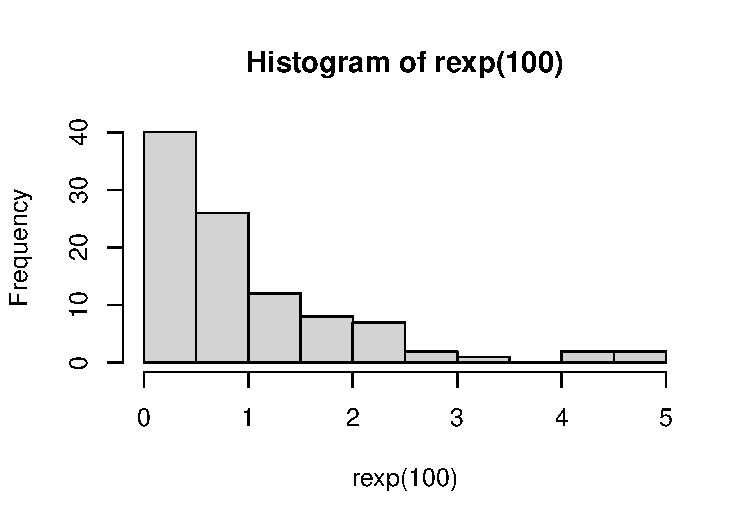
\includegraphics[width=\maxwidth]{figure/unnamed-chunk-6-1} 
\end{knitrout}
\caption{A histogram of random exponentially distributed data, $n=100$.}
\label{plot1} %we can now reference plot1
  \end{center}
\end{figure}

\columnbreak

\subsection{Tables}

\textbf{References}

\pagebreak


%%%%%%%%%%%%%%%%%%%%%%%%%%%%%%%%%%%%%%%%%%%%%%%%%%%%%%%%%%%%%%%%%%%%%%%%%%%%%%%%
% Bibliography
%%%%%%%%%%%%%%%%%%%%%%%%%%%%%%%%%%%%%%%%%%%%%%%%%%%%%%%%%%%%%%%%%%%%%%%%%%%%%%%%
\vspace{2em}

\noindent\textbf{Bibliography:} Note that when you add citations to your bib.bib file \emph{and}
you cite them in your document, the bibliography section will automatically populate here.

\begin{tiny}
\bibliography{bib}
\end{tiny}
\end{multicols}

%%%%%%%%%%%%%%%%%%%%%%%%%%%%%%%%%%%%%%%%%%%%%%%%%%%%%%%%%%%%%%%%%%%%%%%%%%%%%%%%
% Appendix
%%%%%%%%%%%%%%%%%%%%%%%%%%%%%%%%%%%%%%%%%%%%%%%%%%%%%%%%%%%%%%%%%%%%%%%%%%%%%%%%
\onecolumn
\section{Appendix}

If you have anything extra, you can add it here in the appendix. This can include images or tables that don't work well in the two-page setup, code snippets you might want to share, etc.

\end{document}
